\documentclass[journal, onecolumn, a4paper]{IEEEtran}
\usepackage[utf8]{inputenc}
\usepackage{xcolor}
\usepackage{amssymb}
\usepackage{amsmath}
\usepackage{color}
\usepackage{tikz}
\usetikzlibrary{shapes, arrows.meta, positioning}

\begin{document}

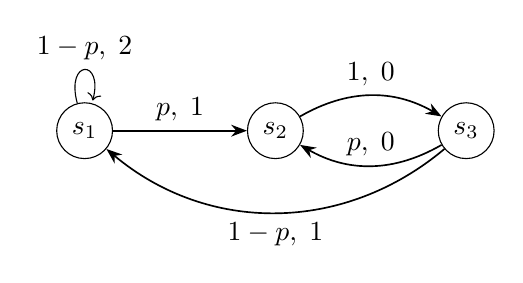
\begin{tikzpicture}[
    node distance=1.7cm,
    state/.style={circle, draw, minimum size=0.5cm},
    transition/.style={-Stealth, semithick}
]

% Nodes
\node[state] (A) {$s_1$};j
\node[state, right=of A] (B) {$s_2$};
\node[state, right=of B] (C) {$s_3$};

% Transitions
\draw[transition] (A) -- node[midway, above] {$p, \; 1$} (B);
\draw[transition] (C) to[out=220,in=320] node[midway, below] {$1-p, \; 1$} (A);
\path (A) edge [loop above] node[midway, above] {$1-p, \; 2$} (A);
\draw[transition] (B) to[out=30,in=150] node[midway, above] {$1, \; 0$} (C);
\draw[transition] (C) to[out=210,in=330] node[midway, above] {$p, \; 0$} (B);
\end{tikzpicture}

\end{document}